\documentclass[titlepage, a4paper]{article}
\usepackage[english]{babel}
\usepackage[utf8]{inputenc}
\usepackage{graphicx}
\usepackage{color}
\usepackage{mathtools}
\usepackage{float}
\usepackage[parfill]{parskip}
\usepackage[margin=10pt,font=small,labelfont=bf,labelsep=endash]{caption}
\usepackage{epstopdf}
\usepackage{listings}
\usepackage[table]{xcolor}
\epstopdfsetup{suffix=}
\DeclareGraphicsExtensions{.ps}
\DeclareGraphicsRule{.ps}{pdf}{.pdf}{`ps2pdf -dEPSCrop -dNOSAFER #1 \noexpand\OutputFile}


\definecolor{green}{rgb}{56,90,115}

\lstset{literate=%
    {å}{{\r{a}}}1
    {ä}{{\"a}}1
    {ö}{{\"o}}1
    {Å}{{\r{A}}}1
    {Ä}{{\"A}}1
    {Ö}{{\"O}}1
}

\newcommand{\todo}[1] {\textbf{\textcolor{red}{#1}}}

\usepackage{fancyhdr}
\fancyhead[L]{}
\pagestyle{fancy}
\rhead{Alexander Yngve \\ Pål Kastman}
\chead{TDTS08}
\thispagestyle{empty}

\begin{document}

{\ }\vspace{45mm}

\begin{center}
  \Huge \textbf{TDTS08: Lab Report}
\end{center}
\begin{center}
  \Large Lab 3: Superscalar Processors
\end{center}

\vspace{250pt}

\begin{center}
  \begin{tabular}{|*{3}{p{40mm}|}}
    \hline
    \textbf{Name} & \textbf{PIN} & \textbf{Email} \\ \hline
           {Alexander Yngve} & {930320-6651} & {aleyn573@student.liu.se} \\ \hline
           {Pål Kastman} & {851212-7575} & {palka285@student.liu.se} \\ \hline
  \end{tabular}
\end{center}
\newpage

\tableofcontents
\thispagestyle{empty}
\newpage

\section{Introduction}\label{sec:intro}
The purpose of this lab is to learn how Supersclar Processors work, and to try and modify a processor architecture to make it simpler, but it should still perform within 5\% of the inital designs performance.


\section{Method}
We started out by investigating every part of the design individually, to see how they affected the performance of the design.

We then choose to simplify the parts that didn't affect the performance. We determined what parts we couldn't simplify due to that the performance would go further than 5\% from the initial performance.

Now we looked at the parts of the design that we could modify, and at their traces.

\section{Result}
In order to establish a baseline performance the simulator was run with the default arguments and a trace was created, with the command shown in listing \ref{sim:simcom}.

\begin{lstlisting}[caption=Simulator command., label=sim:simcom, breaklines=true]
sim-outorder -config superscalar.cfg -ptrace trace.trc 100000:+30 go.ss 3 8
\end{lstlisting}

The config file ''superscalar.cfg'' is supplied with the lab and contains all default settings. The most interesting of these are shown in table \ref{tab:default}.

\begin{table}[H]
\centering
\caption{Default settings.}

\begin{tabular}{|l|r|}
  \hline
  \textbf{Setting} & \textbf{Value} \\ \hline
  res:ialu & 4 \\ \hline
  res:imult & 4 \\ \hline
  res:fpalu & 2 \\ \hline
  res:fpmult & 2 \\ \hline
  ruu:size & 32 \\ \hline
  commit:width & 8 \\ \hline
  issue:width & 8 \\ \hline
  decode:width & 16 \\ \hline
  fetch:speed & 1 \\ \hline
\end{tabular}

\label{tab:default}
\end{table}

Running the simulator with the default settings gave us a simulation time of \textbf{50868222} cycles, with the 5\% requirement from section \ref{sec:intro} this results in a maximum of \textbf{53411633} simulation cycles.

\subsection{Integer components}
\begin{figure}[H]
  \centering
  \scalebox{0.342}{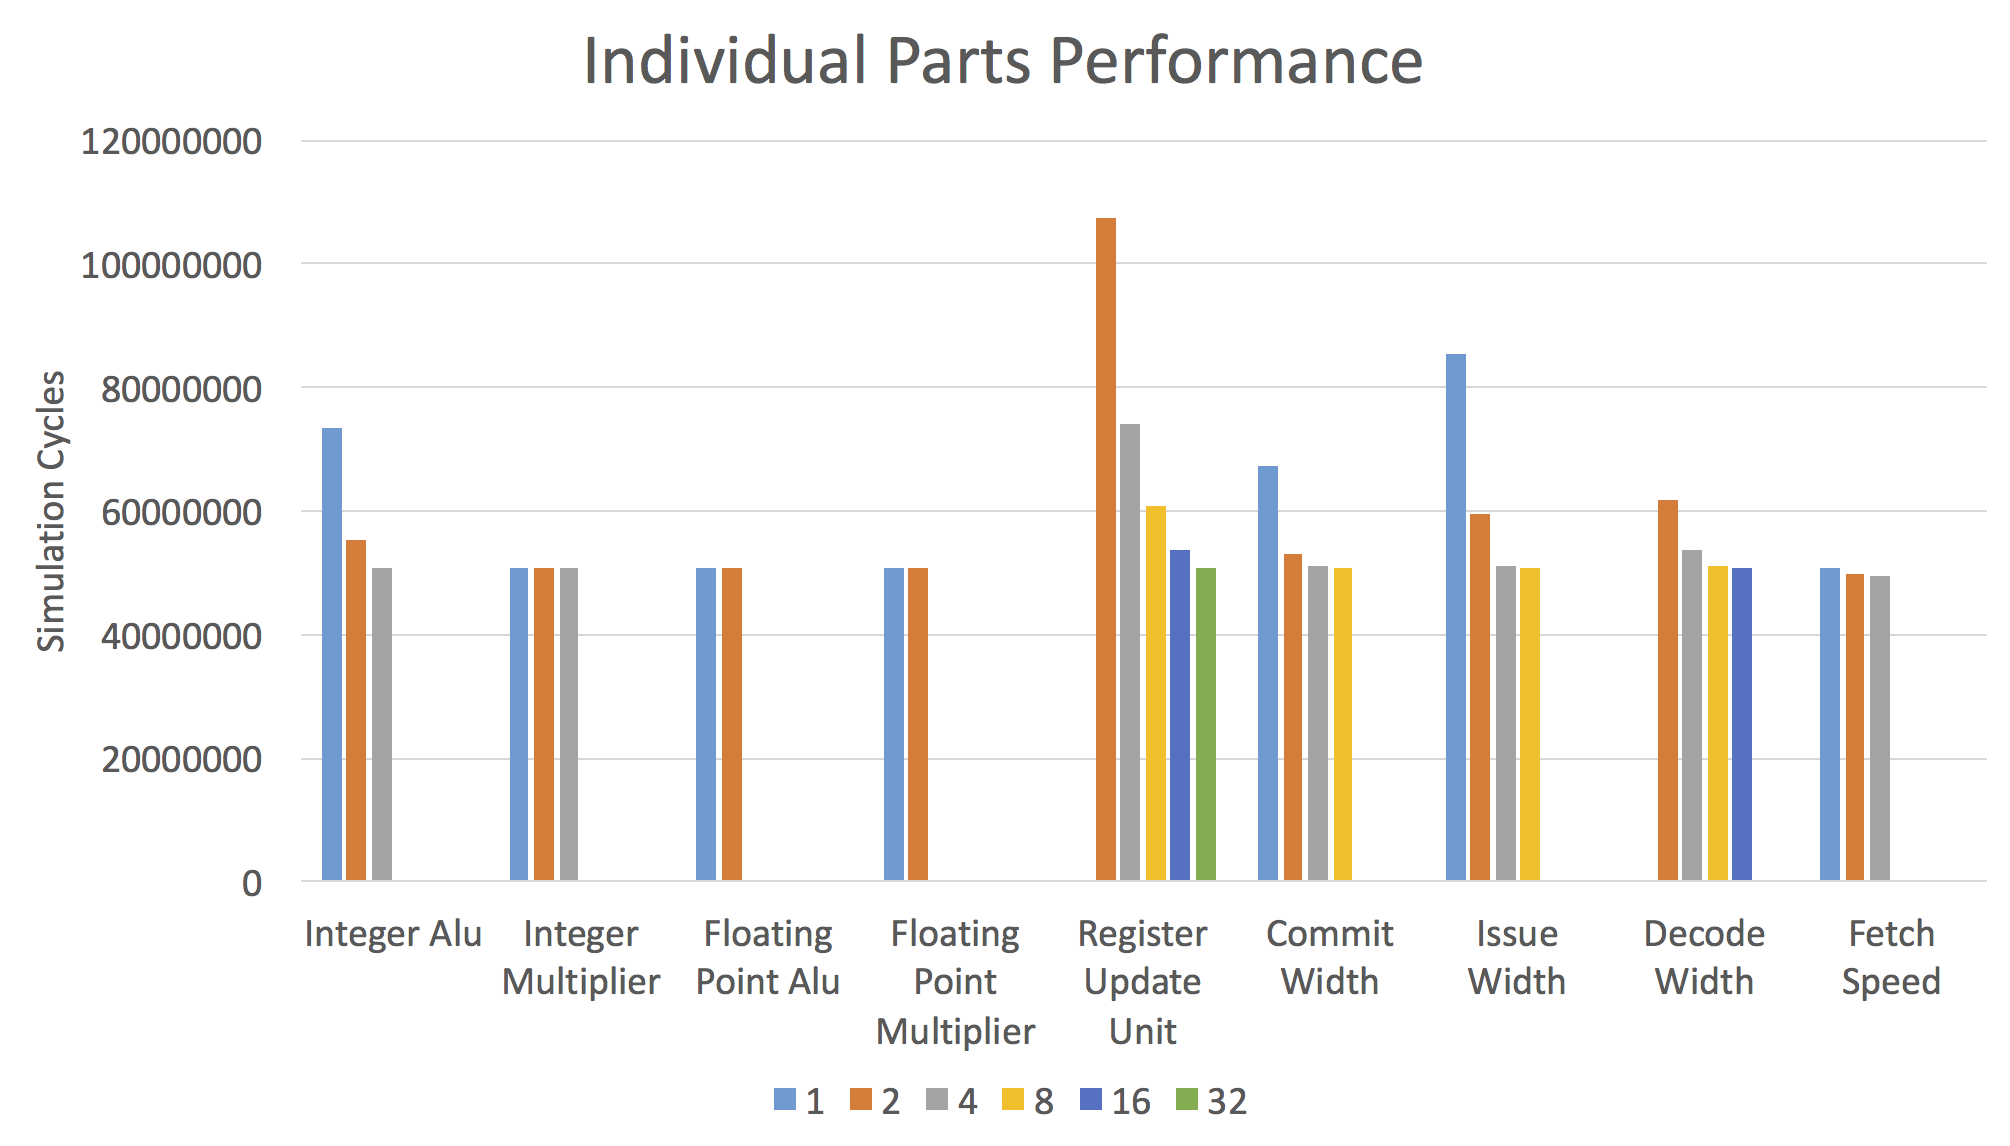
\includegraphics{img/performance.png}}
  \caption{How the individual parts perform.}
  \label{fig:performance}
\end{figure}

In figure \ref{fig:performance} we can see that reducing the number of integer multipliers to only one, no noticeable change in performance could be seen. Therefore we decided to reduce the amount to only one.

\begin{table}[H]
\centering
\caption{Integer settings.}

\begin{tabular}{|l|r|r|}
  \hline
  \textbf{Setting} & \textbf{Value} & \textbf{Simulation cycles}\\ \hline
  res:ialu & 2 & 55360220 \\ \hline
  res:ialu & 1 & 73570279 \\ \hline
  res:imult & 2 & 50868222 \\ \hline
  res:imult & 1 & 50868609 \\ \hline
\end{tabular}

\label{tab:integer}
\end{table}

When observing the Integer alu:s, we instead see in table \ref{tab:integer}, that the performance will reduce drastically when reducing the amount from 4, thus we decided not to change this in the design, as the performance will drop beneath 5\% of the standard design performance.

\subsection{Floating Point components}
In figure \ref{fig:performance} we can see that by changing the floating point alu \& multiplier, the system didn't perform any worse, thus we decided to simplify these as much as possible.

\begin{table}[H]
\centering
\caption{Floating point settings.}

\begin{tabular}{|l|r|r|}
  \hline
  \textbf{Setting} & \textbf{Value} & \textbf{Simulation cycles}\\ \hline
  res:fpalu & 1 & 50868222 \\ \hline
  res:fpmult & 1 & 50868222 \\ \hline
\end{tabular}

\label{tab:floatingpoint}
\end{table}

\subsection{Control components}
The speed of the system was already at the lowest possible, which means by changing this value will increase the complexity of the design, and therefore we decided not to.

When changing the Register Update Unit wee can see in table \ref{tab:control}, that when reducing only one step to 16 instead of 32 we get such a result that by changing this we would nog longer be within 5\% of the standard designs performance.

\begin{table}[H]
\centering
\caption{Control components settings.}

\begin{tabular}{|l|r|r|}
  \hline
  \textbf{Setting} & \textbf{Value} & \textbf{Simulation cycles}\\ \hline
  ruu:size & 16 & 53807041 \\ \hline
  ruu:size & 8 & 60781481 \\ \hline
  ruu:size & 4 & 74098784 \\ \hline
  ruu:size & 2 & 107565825 \\ \hline
  commit:width & 4 & 51076751 \\ \hline
  commit:width & 2 & 53040135 \\ \hline
  commit:width & 1 & 67227355 \\ \hline
  issue:width & 4 & 51187526 \\ \hline
  issue:width & 2 & 59378979 \\ \hline
  issue:width & 1 & 85571238 \\ \hline
  decode:width & 8 & 51165249 \\ \hline
  decode:width & 4 & 53609877 \\ \hline
  decode:width & 2 & 61683477 \\ \hline
  fetch:speed & 4 & 49804290 \\ \hline
  fetch:speed & 2 & 50868222 \\ \hline
\end{tabular}

\label{tab:control}
\end{table}

\subsection{Simplified Design}

\section{Discussion}
For floating point alu \& multiplier we believe that these parts doesn't affect the performance due to that go.ss only uses integer values.

\subsection{Atomic bomb go game}
In Hiroshima, Japan on August 6, 1945, a game of Go was being played. Meanwhile high above the clouds, a lonely B29 Superfortress was soaring peacefully like an Albatross. It was carrying a very special payload, a product of a joint venture between science and military interests. The game was about to enter its third day of play when the B29 dropped an atomic bomb at 8:15am. After the boom the game was continued outside the city due recommendation from the police.

\end{document}
